\chapter{Columnar Storage}
\label{c:columnar-storage}

In this chapter, we explore the application of columnar data structures for different storage components of the \gls{gdbms}, to meet the desiderata we outlined in Chapter~\ref{c:guidelines}. Section \ref{sec:vertex-property-columns} describes the design of columns to store vertex properties and a new compact vertex identification scheme that accompanies the design. In Section \ref{sec:edge-property-columns}, we start by describing the two columnar storage designs to store edge properties and their pros and cons. Then, we propose a third design, \textcolor{red}{paged edge property list}, that is a sweet spot between the earlier two designs and the one we adopt as an optimum design for storing edge properties. Similar to Section~\ref{sec:vertex-property-columns}, we describe a novel and compact edge identification scheme that accompanies our design from edge property columns. \textcolor{red}{As we observed earlier, adjacency lists are already columnar structures.} Section~\ref{sec:adjacency-lists} describes several storage optimizations to the adjacency lists to reduce the system's memory footprint without sacrificing query performance, using the type of structures we observed in guideline~\ref{gdln:graph-schema}.

\section{Columns for Vertex Properties}
\label{sec:vertex-property-columns}

\begin{figure}
	\vspace{-15pt}
	\hfill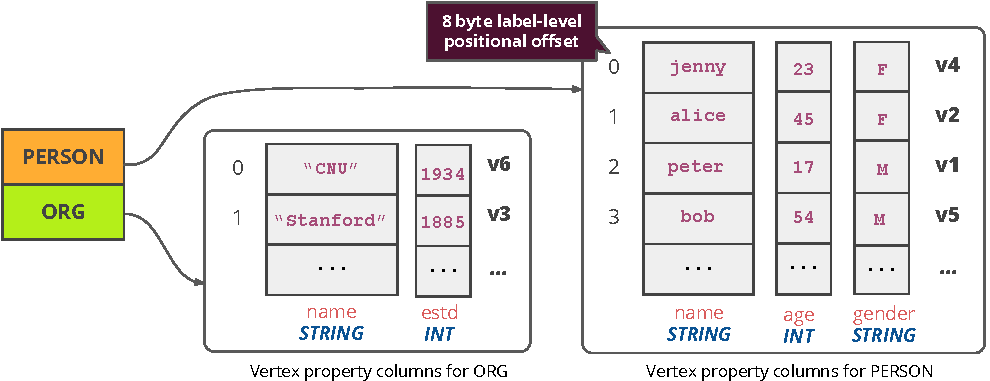
\includegraphics[scale=0.85]{img/vpcols}\hspace*{\fill}
	\caption{Vertex property columns for the graph in Fig.~\ref{fig:runn}.}
	\label{fig:vpcols}
	\vspace{-8pt}
\end{figure}

Columnar data-structures can be directly used for storing vertex properties. Let $(lv_1, lv_2, ...)$ be the vertex labels in a graph. Let $p_{i,1},  p_{i,2}, ... p_{i, n}$ be the structured vertex properties of $lv_i$, with a datatype $d_{i,j}$. We define a \emph{vertex property column}, $CV_{i,j}$, for each $p_{i,j}$, having a fixed data type $d_{i,j}$. Each column stores the value of a single property $p_{i,j}$ for all vertices having $lv_i$ at consecutive locations. The collection of columns of a particular vertex label $lv_i$ is called the column family, $FCV_i$. 

By its structure, a column is a single-dimensional array of \emph{fixed-width} elements. We store one vertex property per element in a column. The property value of a vertex can be directly read using positional offset in the column. Vertex property columns are not ordered, not even by the \texttt{vertexID}. New insertions to a column are performed by simply appending at the end of the column. However, we ensure that all property values of a particular vertex $v$, having label $lv_i$, is located at the same positional offset in their respective columns of the family $FCV_i$. We call this positional offset, \emph{(vertex) label-level positional offset} of vertex $v$. This positional offset can be thought of as the identity of $v$ within its vertex label $lv_i$, that is used to reference properties of $v$. Further, the global identity of $v$ can be given by \textit{(vertex label, label-level positional offset)} pair. 

Figure~\ref{fig:vpcols} shows the set of vertex property columns for the graph in Fig.~\ref{fig:runn}. It has 2 column families, one for each vertex label in the system, with a column for each structured property of the label. The \texttt{vertexID}s on the right of a column family indicates the offset at which the properties of a vertex are located in the columns.

Ideally, the property value of a vertex should directly be read using the ID of the vertex as positional offset in the column. However, \gls{gdbms} typically gives globally unique 8-byte cnsecutive IDs to all the vertices in the system, irrespective of their labels. That means, ID 0 can be given to a vertex with label PRESION and 1 to the vertex with label ORG. We cannot use this ID scheme as the positional offset for the above design. One possible solution is to maintain a map for each label, from the vertex's \enquote{global} ID to its \enquote{local}, i.e, label-level possitional offset of a vertex in the column. This, however, requires extra storage for maintaining the map and an one level of indierction when accessing the vertex properties. Instead, we identify a vertex by a \emph{\textbf{(vertex label, label-level positional offset)}} tuple in the system in place of global vertex ID. This allows direct access to the properties by using the positional offset which now is part of the vertex ID. However, using this new vertex ID scheme requires materializing 2 pieces of information in the adjacency lists - a vertex label and a local positional offset, compared to only global vertex ID by the earlier scheme. This increases the memory overhead as the \enquote{local} positional offsets and the global vertex ID are of the same size. However, as we will show in section \ref{sec:storage-optimizations}, we can often avoid storing the vertex labels with vertex IDs and even save space by using fewer bytes for local positional offsets than the bytes needed by the global vertex IDs.



\section{Columns for Edge properties}
\label{sec:edge-property-columns}

From \ref{ssec:edges-ordered}, we know that 1) edges are read by the \texttt{JOIN} operators in the order they appear in the adjacency lists, and, 2) edge properties are read in the order in which edges are read from the adjacency lists. This calls for storing edge properties in the order of edges. To localize reading edge properties, each edge proerty has to be replicated twice with each appearance of the edge, once in the forward adjacency list of edge's source vertex and then again in the backward adjacency list of the destination vertex. We present two naive solutions, that can be seen as opposite ends of the spectrum, optimizing the system for \emph{storage} and \emph{performance} respectively:

\begin{figure}
	\vspace{-25pt}
	\hspace*{-20pt}
	\begin{subfigure}{0.45\textwidth}
		\vspace{8pt}
		\centering
		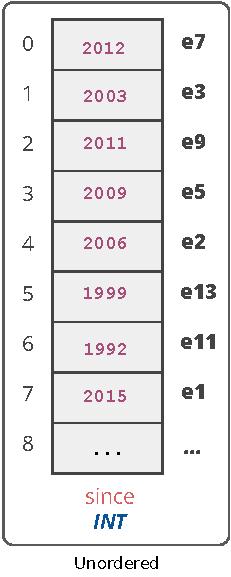
\includegraphics[scale=0.8]{img/sol1}
		\captionsetup{justification=centering}
		\caption{Sol 1: (Unordered, No Replication)}
		\label{fig:sol1}
	\end{subfigure}
	\begin{subfigure}{0.55\textwidth}
		\centering
		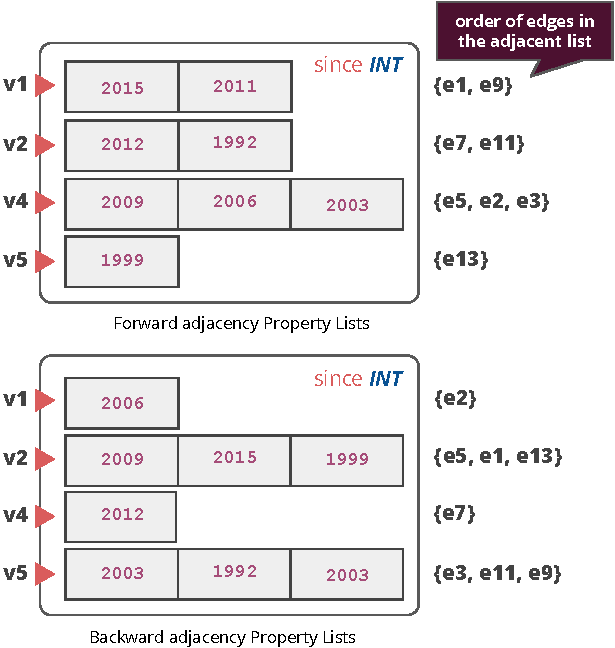
\includegraphics[scale=0.8]{img/sol2}
		\captionsetup{justification=centering}
		\caption{Sol 2: (Ordered, Replication)}
		\label{fig:sol2}
	\end{subfigure}
	\captionsetup{justification=centering}
	\caption{Edge property columns in Solution 1 and 2 for \texttt{since} property in Fig.~\ref{fig:runn}.}
	\label{fig:sol1and2}
	\vspace{-8pt}
\end{figure}

\vspace{-12pt}
\subparagraph{Solution 1: (Unordered, No replication) } This solution optimizes for storage since each property is stored once in the system. We use the same design as that for storing the vertex properties. That is, we have one unordered edge property column for each $q_{i,j}$, where $q_{i,j}$ is a structured property of edge label $l_i$. Edges in the system with this solution can be identified as \emph{(edge label, label-level positional offset)}. However, such a design would be oblivious to the fact that edges and their properties are accessed in order. Reading the edge property value is random access to these columns. Therefore, the queries cannot benefit from cache locality which would have been there if edge property values were stored together. As a secondary disadvantage, an edge will be stored in 12 bytes (4-byte label, 8-byte offset) in adjacency lists, compared to 8 bytes per edge earlier.

Figure~\ref{fig:sol1} shows the edge property column for edgel label \texttt{FOLLOW}'s \texttt{since} property. Property values are not ordered. For our running example, the forward adjacency list of \texttt{v4} contains edges \texttt{e5}, \texttt{e2} and \texttt{e3}, whose \texttt{since} property value (at positional offsets 3, 4 and 1) in the edge property column is not stored together. 

\vspace{-12pt}

\subparagraph{Solution 2: (Ordered, Replication) } This solution replicates each edge property value twice but offers reading the edge property values sequentially in all scenarios. We keep two \emph{oredered} edge property columns for each $q_{i,j}$, we callthem \emph{forward adjacency list-ordered} and \emph{backward adjacency list-ordered}. Property values in forward adjacency list-ordered column are grouped by their edge's source vertex and ordered by source vertex's forward adjacency list. Similarly, the property values in the backward adjacency list-ordered column are grouped by the edge's destination vertex and ordered by the destination vertex's backward adjacency list. This way, a query that is reading an adjacency list of a vertex $v$, reads the adjacent edges' property value sequentially from the relevant group of same-ordered edge property column. This solution also comes with an advantageous side effect. We can completely get rid of storing any edge identifier in the adjacency lists; instead, we just store the pointer to the relevant groups of columns with each adjacency list. Then, the location of property value can be obtained by using the pointer to the relevant group and the positional offset of the edge in adjacency list. Lastly, updates become tough as each property value now has to be inserted in 2 columns.

Figure~\ref{fig:sol2} shows the forward and backward adjacency list-ordered edge property columns for edgel label \texttt{FOLLOW}'s \texttt{since} property. For our running example, the forward adjacency list of \texttt{v4} contains edges \texttt{e5}, \texttt{e2} and \texttt{e3}, whose \texttt{since} property appear together in the forward adjacency list-ordered (right) column in the figure. Hence, the properties of the edges in an adjacency list are always sequentially read.

\subsection{Vertex-grouped Edge Property Columns}

Solutions 1 and 2 present extreme cases for optimizing storage and performance, respectively. This solution presents the middle ground. The idea is to avoid replication of property values while not completely losing cache locality benefits that we get from reading values from column sequentially. Hence, we keep any one of the two columns we had for each property $q_{i,j}$ in Solution 2.

We define an \emph{ordered} edge property column, $CE_{i,j}$, for each edge property $q_{i,j}$. The collection of columns having the label $le_{i,j}$ forms a family $FCE_i$ and are either forward or backward adjacency list-ordered. If a family $FCE_i$ is forward adjacency list-ordered, it means that all property values of an edge $e$, having label $le_i$, are grouped by the edge's source vertex and ordered by source vertex's forward adjacency list in columns of $FCE_i$; and similarly if a family for backward adjacency list-ordered column. The property values grouped by source or destination vertex is called a \emph{vertex group} in a column. Property values of $e$ are further located at the same positional offset across all columns of $FCE_i$. Reading from an edge property column that is forward adjacency list-ordered is sequential if the edges are read from a vertex's forward adjacency list. However, if the edges are read from the backward adjacency list, the property values have to be accessed randomly out-of-order.

\begin{figure}
	\vspace{-25pt}
	\hfill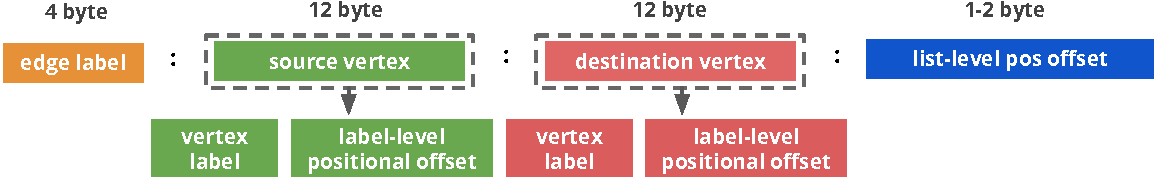
\includegraphics[scale=0.78]{img/edge-scheme}\hspace*{\fill}
	\captionsetup{justification=centering}
	\caption{Components of the new Edge identification scheme.}
	\label{fig:edge-scheme}
	\vspace{5pt}
\end{figure}

The need for randomly accessing property values means that edge identifier cannot be omitted from storing in adjacency lists. A property of edge $e$ having label $le_i$ can be accessed in a vertex-grouped edge property column by knowing 1) $q_{i,j}$; 2) the vertex on which property values in the column are grouped i.e, either source or destination vertex of $e$), and 3) group-level positional offset of $e$. Owing to issues similar to those faced with using \texttt{vertexID} for fetching vertex properties, we adopt a new scheme for identifying edges in the system. The new scheme identifies an edge by a set of following components: \textbf{\emph{(edge label, source vertex, destination vertex, group-level positional offset)}}. This scheme gives tremendous opportunity for reducing the memory footprint of storing edges in the adjacency lists, apart from easily accessing edge property columns. We describe the storage of edges using the new scheme in Section~\ref{sec:storage-optimizations}.

\subsection{Paged Edge Property Columns}
\label{sec:paged-edge-property-columns}

Vertex-grouped edge property columns is a good solution for storing edge properties but are practically infeasible to maintain in the system. We discuss the limitations of vertex-grouped edge property columns and then propose simple modifications to address those limitations. We call the modified solution, paged edge property group, that removes ordering and groups the property values in a column at a memory page-level instead of vertex-level.

\vspace{-12pt}
\subparagraph{Limitations of Vertex-grouped Edge Property Columns.}
Storing edge properties in vertex-grouped edge property lists are not update friendly owing to the existence of strict ordering in each group of all the columns. For example, assume a scenario where a new edge is has to be inserted at \emph{position 5} in a forward adjacency list $A$ of vertex $v$ having a size \emph{10}. The vertex groups of $v$ that are ordered by $A$ will have to undergo shifting to make space for the properties of new edge at position 5. This will modify the list-level positional offsets of edges appearing at positions $\geq 5$ in $A$. Changing the positional offsets of modified edges is costly since it requires $n$ traversals of adjacency lists, where $n$ is the number of modified edges. Hence, each edge insertion will cause physical changes to the columns as well as multiple adjacency lists.

Apart from costly insertions, maintaining pointers to each of the group in all the columns introduces significant memory overhead. 

\vspace{-16pt}
\subparagraph{Modifications.}
To make insertions easy, we omit the proposition of strict ordering in each vertex group of columns. By giving up ordering, queries no longer read the edge property values sequentially while extending from the adjacency list on which the group is ordered. However, we are still able to maintain cache locality by reading the property values from \emph{close-by} locations of a column.

We map $n$ ordered vertex groups from a vertex-grouped edge property column into one unordered page in paged edge property column. This way, a single page holds the property values from $n$ vertex groups. The mapping between vertex groups and page of respective columns is straightforward. Vertex groups of vertices having label-level positional offset $p$ maps to the $p/n$th page in the column. The main benefit of the paged edge property column comes from the fact that it is unordered. Hence, new edge insertions become easy as they get appended into relevant paged edge property column similar to how insertions happen in vertex property columns~\ref{sec:vertex-property-columns}. Property values in a page are still referenced by the group-level positional offset in the new edge identification scheme. However, group-level positional offset in paged edge property column no longer refers to the position of an edge in the ordering adjacency list. Now, the group-level positional offset only refers to the position of properties of an edge in paged edge property columns of a family. 

\begin{figure}
	\vspace{-40pt}
	\hfill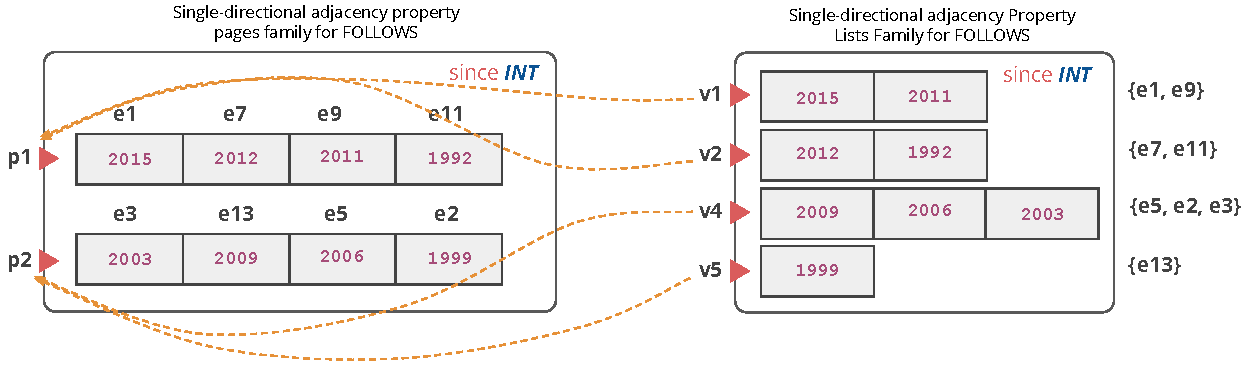
\includegraphics[scale=0.78]{img/paged}\hspace*{\fill}
	\captionsetup{justification=centering}
	\caption{Mapping the Vertex-grouped edge property column to the Paged edge property column for since property in Fig.~\ref{fig:runn}.Here, $n=2$.}
	\label{fig:paged}
	\vspace{-5pt}
\end{figure}

Figure~\ref{fig:paged} shows the mapping of a vertex-grouped edge property column to a paged edge property column for $n=2$. The paged edge property column has two pages that stores the property values from vertex groups $(v1,v2)$ and $(v3,v4)$ respectively.

The driving goal is to choose $n$ such that property values of edges in a defining adjacency list are not too sparse for a cache miss to occur with \emph{each} access of a value. Hence, the value of $n$ is heavily dependant on many factors like the cache line size, column element width and the average number of edges in the adjacency lists in the system. We choose the value of n in the range $32, 512$. We show in experiments that our solution is not significantly worse than the vertex-grouped edge property column when performing sequential reads. Comparing the two, we get a minimal overhead of 1.2x on read-intensive workloads. However, with completely unordered edge property column, the overhead over vertex-grouped edge property columns is as high as 4.5x.

\section{Adjacency Lists as a Column Store}
\label{sec:adjacency-lists}

The adjacency lists can be defined as a data-structure that maps a vertex $v$ to the list of $v$'s adjacent edges and neighbour vertices. Given a vertex $v$, t




\section{Storage optimizations}
\label{sec:storage-optimizations}

In this section, we present ideas on how our storage benefits (in terms of reducing the memory footprint) from the new identification schemes and structures that the data-structures introduced in previous sections. Our optimizations are critical in achieving high-levels of compactions while storing edges in the adjacency lists, thereby reducing the overall memory footprint of data in the system.

\subsection{Removing unnecessary edge information.}

The new edge identification scheme is \emph{virtual}. We do not need to store all the 4 components of the new edge identifier. While iterating on an adjacency list, the edge label of adjacent edge $e$ and the extending vertex ($e$'s source vertex in forward adjacency list and it's destination vertex in backward adjacency list) are already known and hence are not stored in the list. The neighbouring vertex ($e$'s destination vertex in forward adjacency list and source vertex in backward adjacency list) identifier is stored from prior. Therefore, the only storage overhead is the group-level positional offset. The offset is often not more than 1 or 2 bytes. This follows from the fact that the number of edges in most of the adjacency list is very small (by the power-law). Hence, storing the group-level positional offsets as a variable-width element saves memory by 2-3x. Moreover, in many cases, even group-level positional offsets can be omitted from storing in adjacency lists. We look at these cases in \ref{sec:storage-optimizations}.

At the time we introduced the new edge identification scheme in \ref{sec:edge-property-columns}, we briefly discussed the size of storing each edge in the adjacency lists. Out of 4 components in the new edge identifier, only 2 components, \emph{(neighbouring vertex, page-level positional offset)}, are needed to be stored per edge in the adjacency list. Note that the neighbouring vertex itself comprises of 2 components: \emph{(vertex type, type-level positional offset)}. Given that the vertex identifier is 12 bytes and page-level positional offset can be stored in 1 or 2 bytes, storing an edge in an adjacency list takes 14 bytes. We can omit to store the few components of the edge in the following cases: 

\begin{itemize}
	\item \textbf{Neighbouring vertex's type can be omitted while storing edges if it can be inferred implicitly.} We know by \ref{ssec:graph-schema}, that an edge label $l$ has a fixed set of source vertex types and destination vertex types. Using this, we can infer the \emph{probable set} of neighbouring vertex types, $T_N$, while extending a vertex. $T_N$ is defined as the set of vertex types whose vertices an extending vertex can extend to.

	Note that during the \texttt{E/I} operation, we already know, 1) the extending vertex, 2) \emph{direction} of extend, and 3) the edge label of edge we want to extend to. $T_N$ can be determined from the edge label and the direction of extend. If direction of extend is forward, $T_N$ is the destination vertex types of the edge label. Similarly, if direction is backward, source vertex types of the edge label forms $T_N$. 
	
	For cases when $|T_N|$ is $1$, the neighbouring vertex type in our extend operation is fixed. In these case, there is no need to store the neighbouring vertex types with \emph{all} the edges in adjacency list - and can be determined from the graph's schema. The following rules assist the omission of neighbour vertex types while storing edges:
	
	\begin{itemize}
		\item If edge label $l$ has only a source vertex type, then an edge $e$, from vertex $u$ to $v$ and having label $l$, can be stored without the neighbour vertex type in the backward adjacency lists of $v$.
		
		\item Similarly, if edge label $l$ has only a destination vertex type, then an edge $e$, from vertex $u$ to $v$ and having label $l$, can be stored without the neighbour vertex type in the forward adjacency lists of $u$.
	\end{itemize}

    \item \textbf{Edges that do not have properties, do not need page-level positional offsets.} From section \ref{sec:edge-property-columns} and \ref{sec:page-level-edge-property-columns}, we know that an edge's positional offsets is required \emph{only} while accessing its properties' value from relevant page-level edge property columns. Hence, in the absence of any properties on an edge, the (page-level) positional offset of that edge is undefined. Such edges are stored in the adjacency lists without any positional offsets information. In the absense of page-level positional offset, an edge cannot be identified globally since there can be multiple edge with unique \emph{(edge label, source vertex, destination vertex)} tuple. We reason that there is no requirement for an edge to be \emph{identifiable} in the system if not for accessing its properties. Conventionally, the purpose an  \texttt{edgeID} has been two-fold, 1) to connect source and destination vertices and, 2) to reference edge properties (if present). We are able to still fulfill 1) by not having a page-level positional offset while 2) stands void in the absence of properties. 
	
\end{itemize}

\subsection{Fixed-length null suppression}

The components of an edge identifier, usually, do not occupy the entire-width allocated to them in storage. For instance, a neighbouring vertex type is stored as a fixed 4-byte value in the adjacency lists. Likewise, neighbouring vertices' type-level positional offsets do not often exhaust the whole of 8 bytes allocated to them in storage. Clearly 


\subsection{Vertex property columns for single cardinality labels.}

Single cardinality labels are edge labels that have one of the following cardinalities, 1) 1..1 (one-to-one), 2) 1..n (one-to-many), and 3) n..1 (many-to-one). Such labels guarantee that there will be at most a single edge from the source vertex or to the destination vertex. For instance, let us consider an edge label BIRTHDAY that connects a vertex of type PERSON to the vertex of type DATE. Cardinality of BIRTHDAY is \emph{many-to-one}. That is, a vertex PERSON is connected to only one vertex of type DATE, while a vertex DATE can have connections to multiple PERSONs through the edge of label BIRTHDAY.

Single cardinality labels provide the opportunity of optimizing how the edges of such labels are stored. We use the fact that an edge $e$ of a single cardinality label is the \emph{only} element in either the forward adjacency list of $e$'s source vertex or forward adjacency list of $e$'s destination vertex or both. 

...
